 A custom PCIe card developed by the ALICE collaboration, the Common ReadOut Receiver Card (C-RORC) \cite{alice}, was deployed as an 
upgraded detector readout interface within the ATLAS ROS with ATLAS specific firmware and software called the RobinNP \cite{crorc}. 
The new PC based RoIB uses the RobinNP firmware and a dedicated API to facilitate the implementation of the RoIB functionality 
on a commodity PC. In this section, we describe the C-RORC hardware as well as the RobinNP firmware, API, and the event building software. 
\subsection{The Common Readout Receiver Card}\label{sec:crorc}

The C-RORC implements 8 PCIe Gen1 lanes with 1.4 GB/s bandwidth to the CPU fed via 12 optical links each running 200 MB/s on 3 QSFP transceivers. It utilizes a single Xilinx Virtex-6 series FPGA that handles data input from the 12 links and buffers the data in two on-board DDR3 memories. It is also capable of processing and initiating DMA transfer of event data from the on-board memory to its host PC's memory. The major components of the C-RORC are annotated 
in the picture shown in Figure \ref{fig:crorc}.


\begin{figure}[tbp] % figures (and tables) should go top or bottom of
                    % the page where they are first cited or in
                    % subsequent pages
\centering
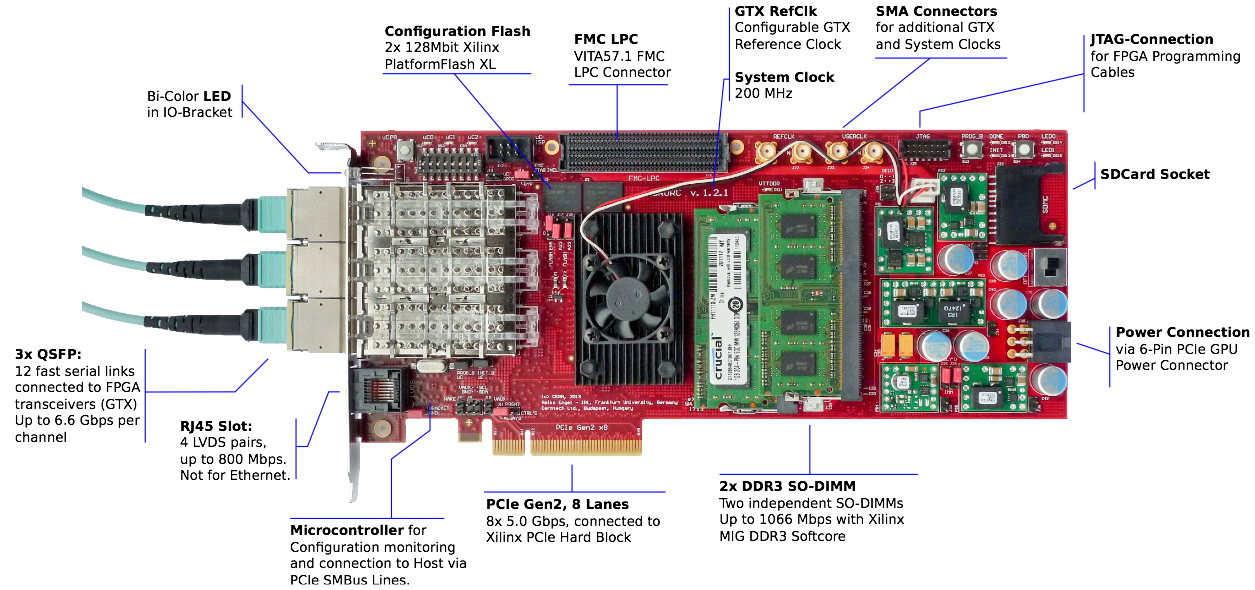
\includegraphics[width=\textwidth]{crorc.png}
\caption{Photo of the C-RORC board with the major components and features annotated \cite{crorc}.}
\label{fig:crorc}
\end{figure}

\begin{figure}[tbp] % figures (and tables) should go top or bottom of
                    % the page where they are first cited or in
                    % subsequent pages
\centering
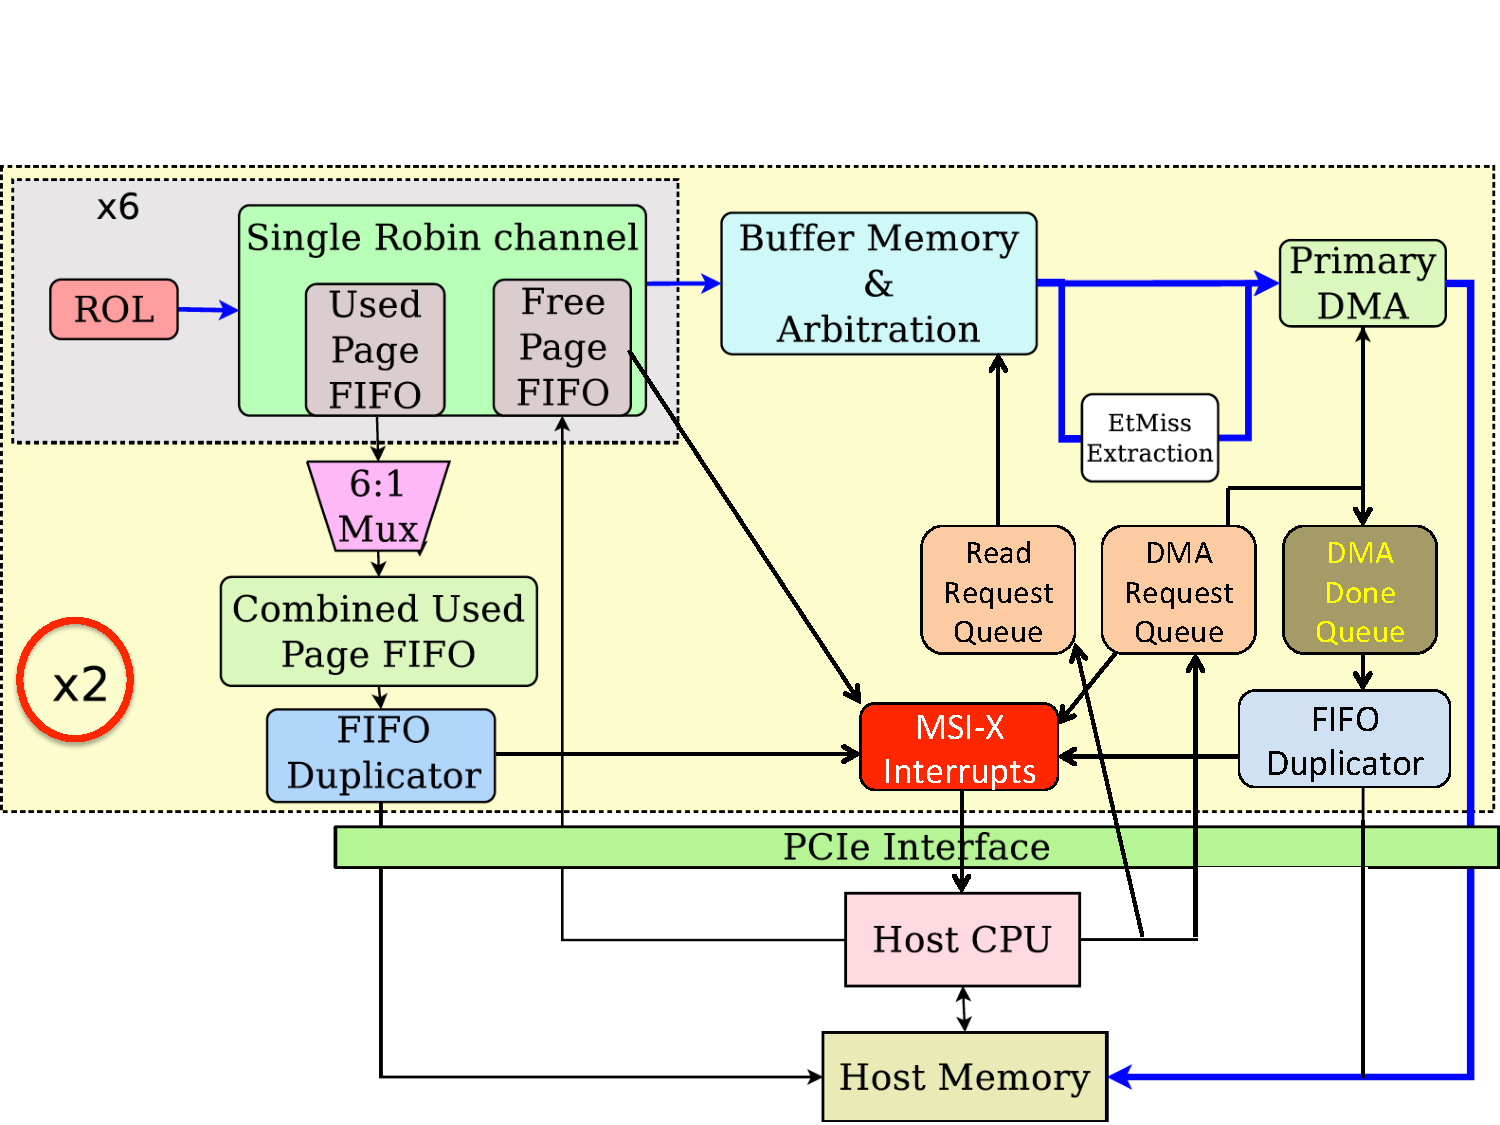
\includegraphics[trim = 0cm 0cm 0cm 2.5cm, clip, width=.71\textwidth]{RobinNP_Firmware}
%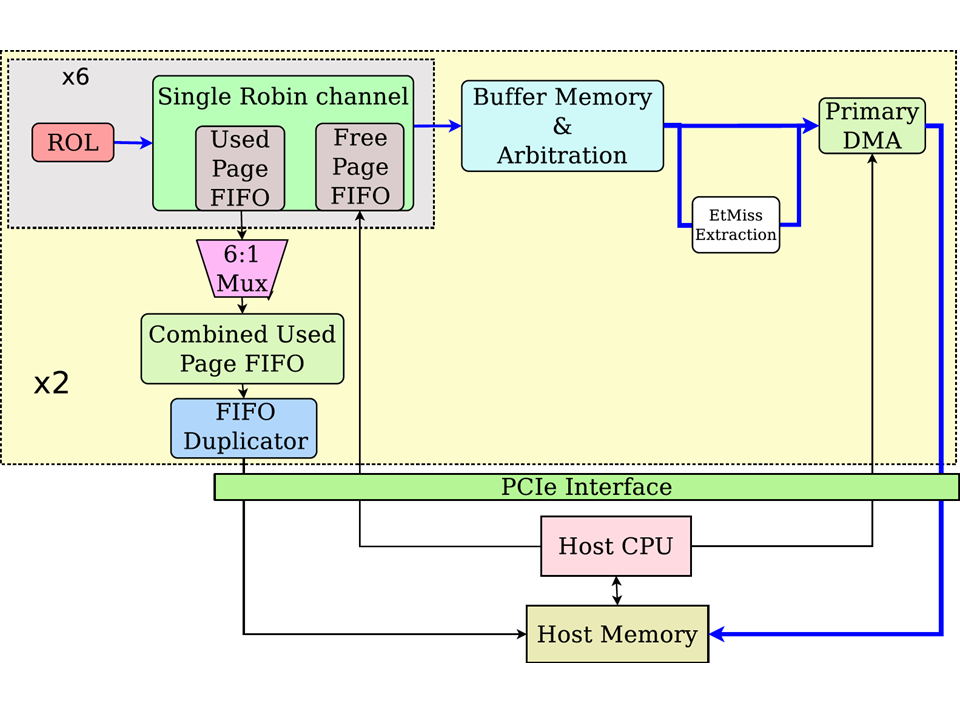
\includegraphics[width=.6\textwidth]{Firmware.jpg}
%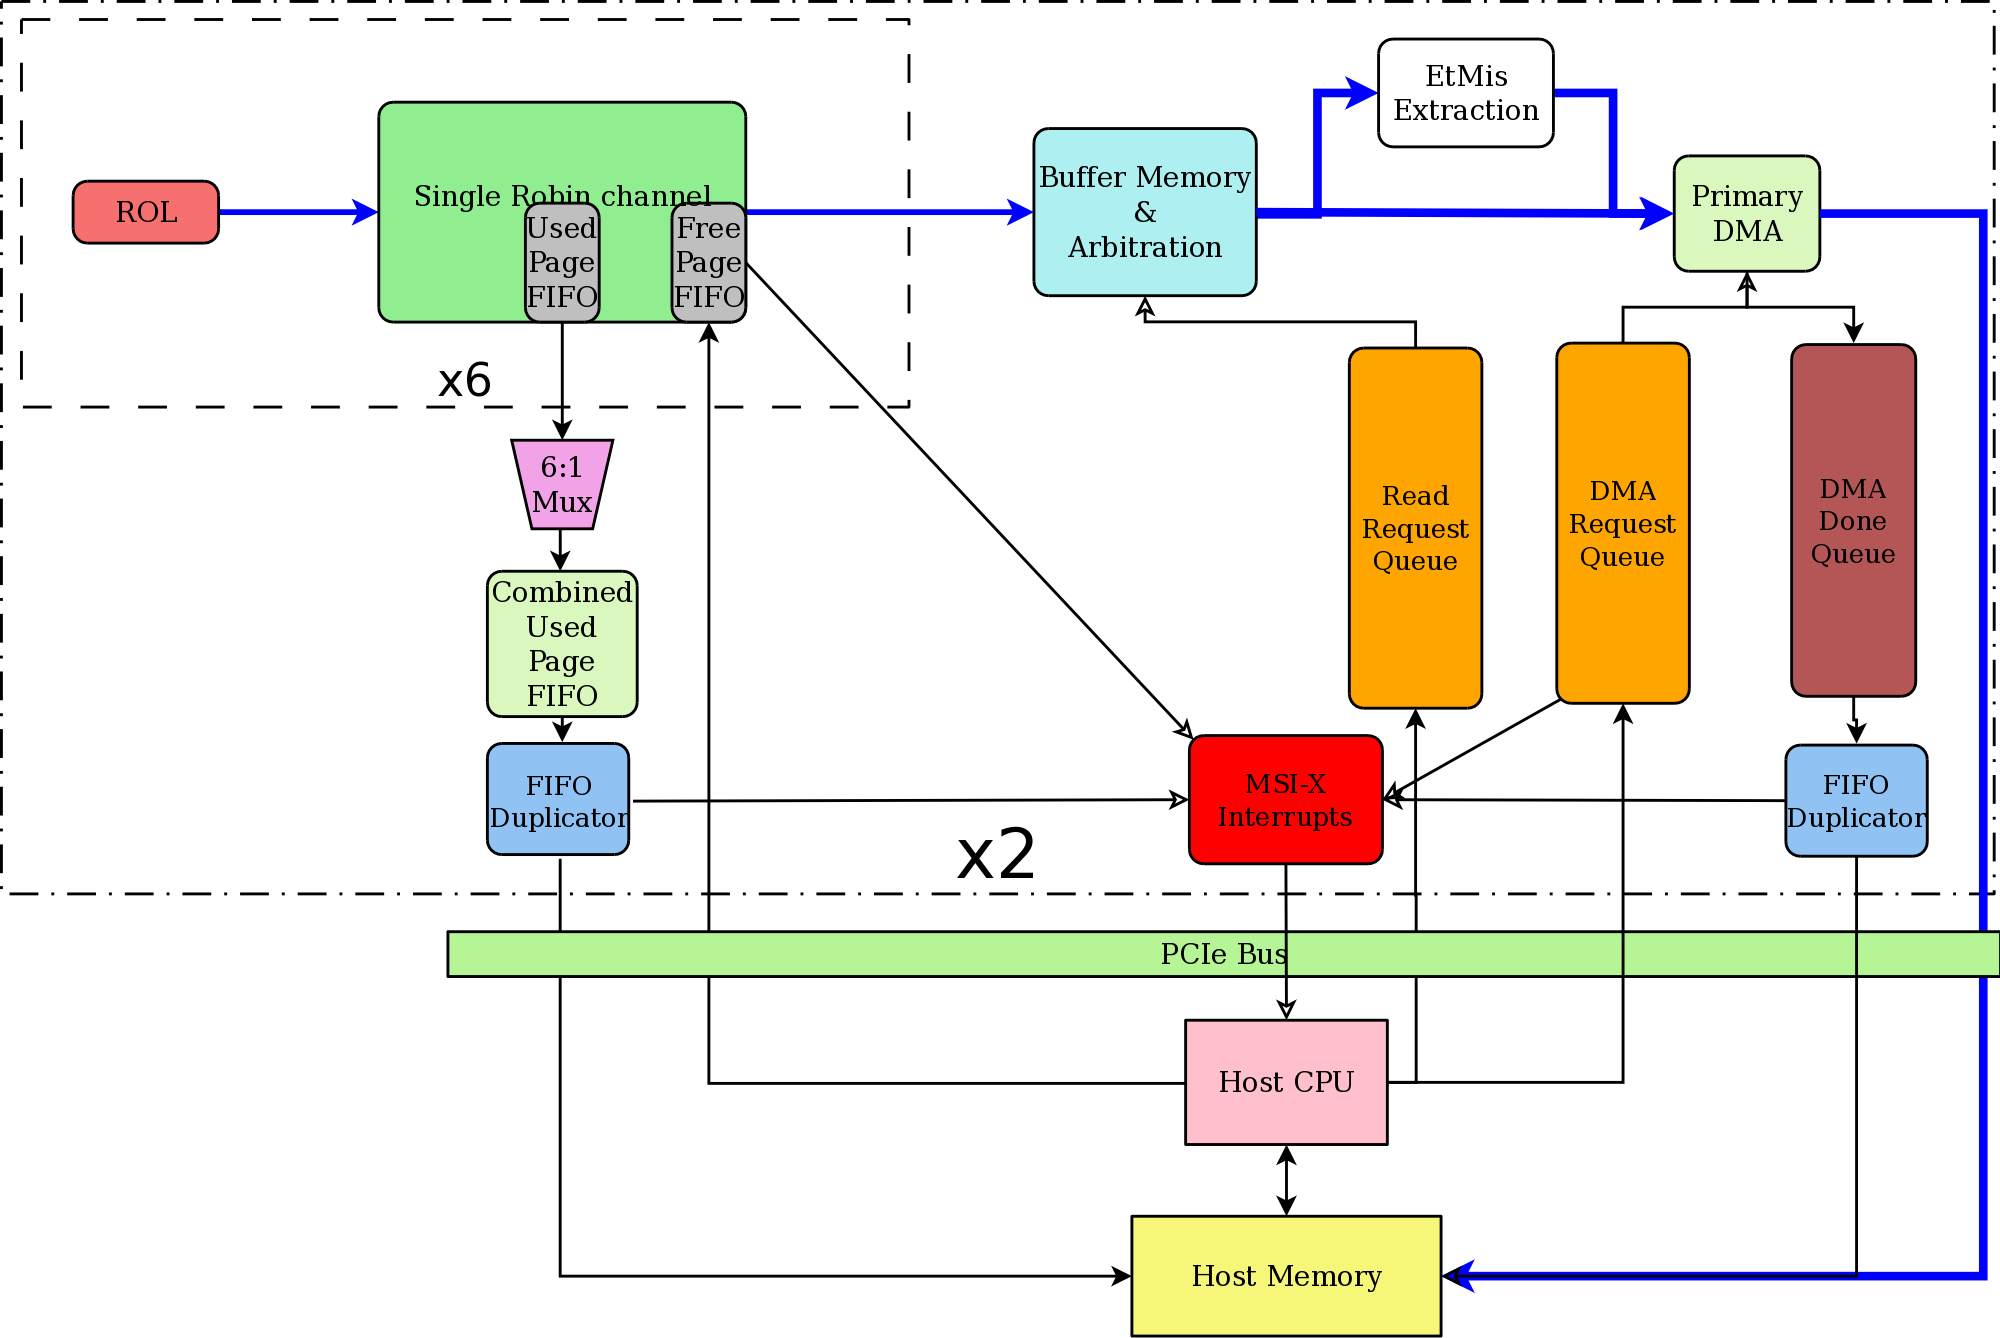
\includegraphics[width=.8\textwidth]{AReducedBlockDiagram.png}

\caption{RobinNP firmware organization
and  flow  of  data  from  host  CPU  to  the
firmware  (by  means  of  programmed  I/O)
and from the firmware to the host memory
(by means of DMA).}
\label{fig:robinnp_fw}
\end{figure}

\subsection{Readout System Firmware \& Software}\label{sec:crorc_fw}

The RobinNP firmware used for the RoIB is identical to that used in the ATLAS ROS\cite{ros}. As shown in 
the schematic of Figure \ref{fig:robinnp_fw}, the logic is divided into two functional blocks, known as sub-ROBs, 
each servicing six input links and one DDR3 memory module. Event data fragments arriving via a link are subjected 
to a range of error checks before being stored in the memory module for the relevant sub-ROB. At the same time a token
representing the address of a region of the memory, referred to as a page, is passed to a listening software process via 
a `FIFO duplicator'. To avoid a costly read across the PCIe bus, data is continuously streamed from firmware to 
software via a chain of firmware and software FIFOs. Notification of new data arriving in the software FIFO is managed via coalesced 
interrupts to allow for efficient use of CPU resources.
For the RoIB application, the receipt of page information immediately triggers a DMA of fragment data from the RobinNP memory into 
the host PC memory. The fragments are then passed via a queue (one per sub-ROB) to the RoIB process along with any relevant fragment 
error information. A schematic of this shortened dataflow path is presented in Figure \ref{fig:roib_swfw}. 
The API for the RoIB process consists of these queues, return queues for processed pages now available for re-use and 
a configuration interface. The software is implemented with multiple threads each handling specific tasks such as supply of free pages, receipt
of used pages, DMA control and bulk receipt of fragment data.


\begin{figure}[tbp] % figures (and tables) should go top or bottom of
                    % the page where they are first cited or in
                    % subsequent pages
\centering
%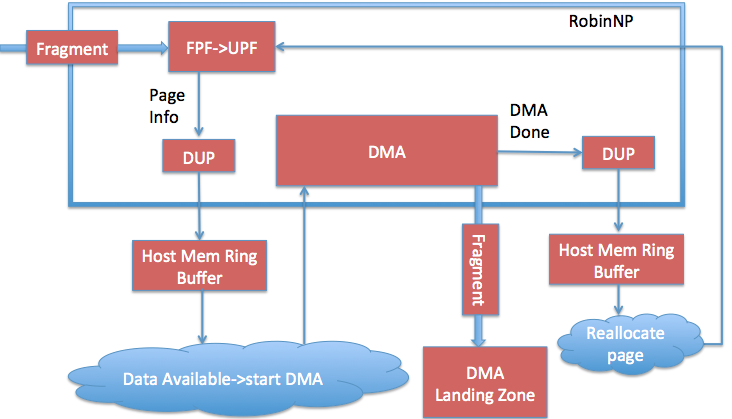
\includegraphics[width=.6\textwidth]{roib_firmware.png}
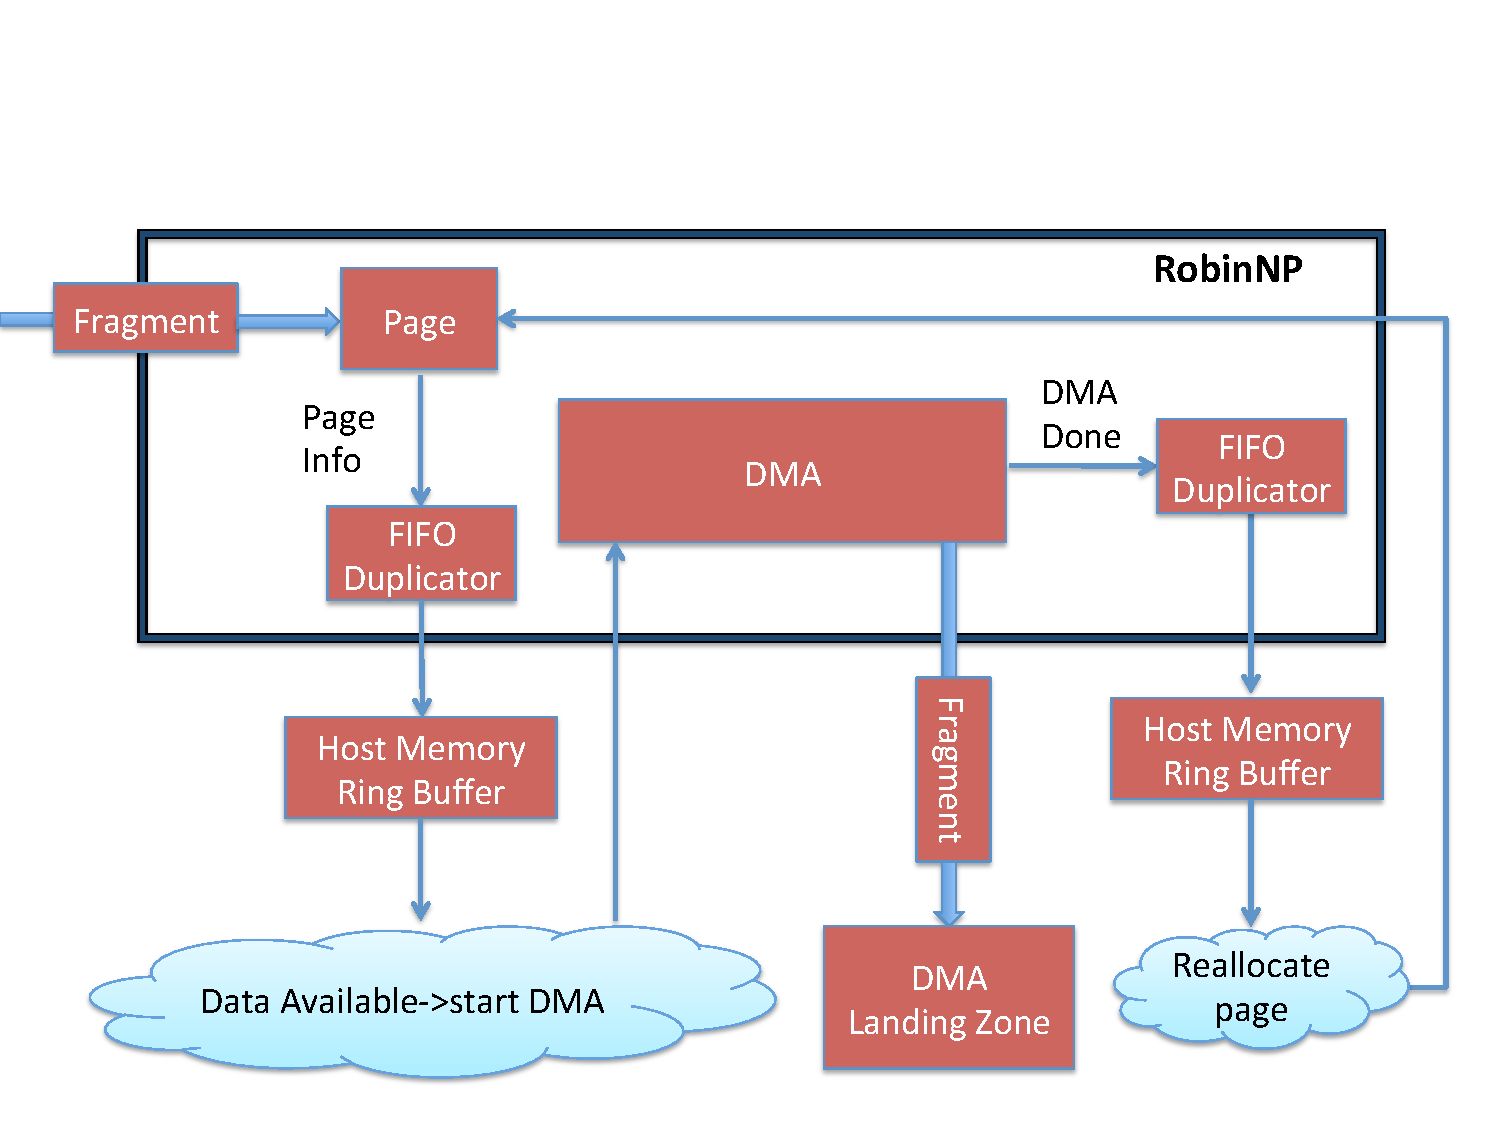
\includegraphics[trim = 0cm 0cm 0cm 5cm, width=.7\textwidth]{RobinNP_Software}
\caption{Layout of the readout system firmware and software specific to the RoIB.}
\label{fig:roib_swfw}
\end{figure}

\subsection{RoIB Software}\label{sec:crorc_sw}

The HLTSV is a multi-threaded application that obtains a L1 result from a variety of possible input sources and exchanges information with the 
rest of the HLT computing farm. 
%Data Collection Managers (DCM). The DCM is the application running on each HLT computing node that tells the HLTSV if the event has been rejected, successfully built, or timed out and also requests the data from the ROS. In this case, 
For the RoIB, the L1 source is a RobinNP interface that performs fragment assembly and is used as a plug-in to the HLTSV application.
The RobinNP plug-in has two receive threads, each 
thread services six channels by pulling fragments from the RobinNP on-board memories to the host PC.
Fragments with the same L1ID are copied 
to a contiguous memory space and a queue of completed events is prepared. 
Upon request by the HLTSV, a pointer to the contiguous memory space is passed back to the 
HLTSV process for further handling. In order to optimize concurrent access to RoIB data structures, containers from the  Intel 
threading building block (TBB) library were used. These containers allow multiple threads to concurrently access and update items 
in the container while maintaining high performance.  
